% ===========================================================================
% IEEE Two-Column LaTeX Figure Environments
% Project: Task-Adaptive Architecture Optimization for LLM-Based Multi-Agent Systems
% ===========================================================================

% --- FIGURE 1: Neural Adaptation Trajectories (Two-column wide figure) ---
\begin{figure*}[t]
\centering
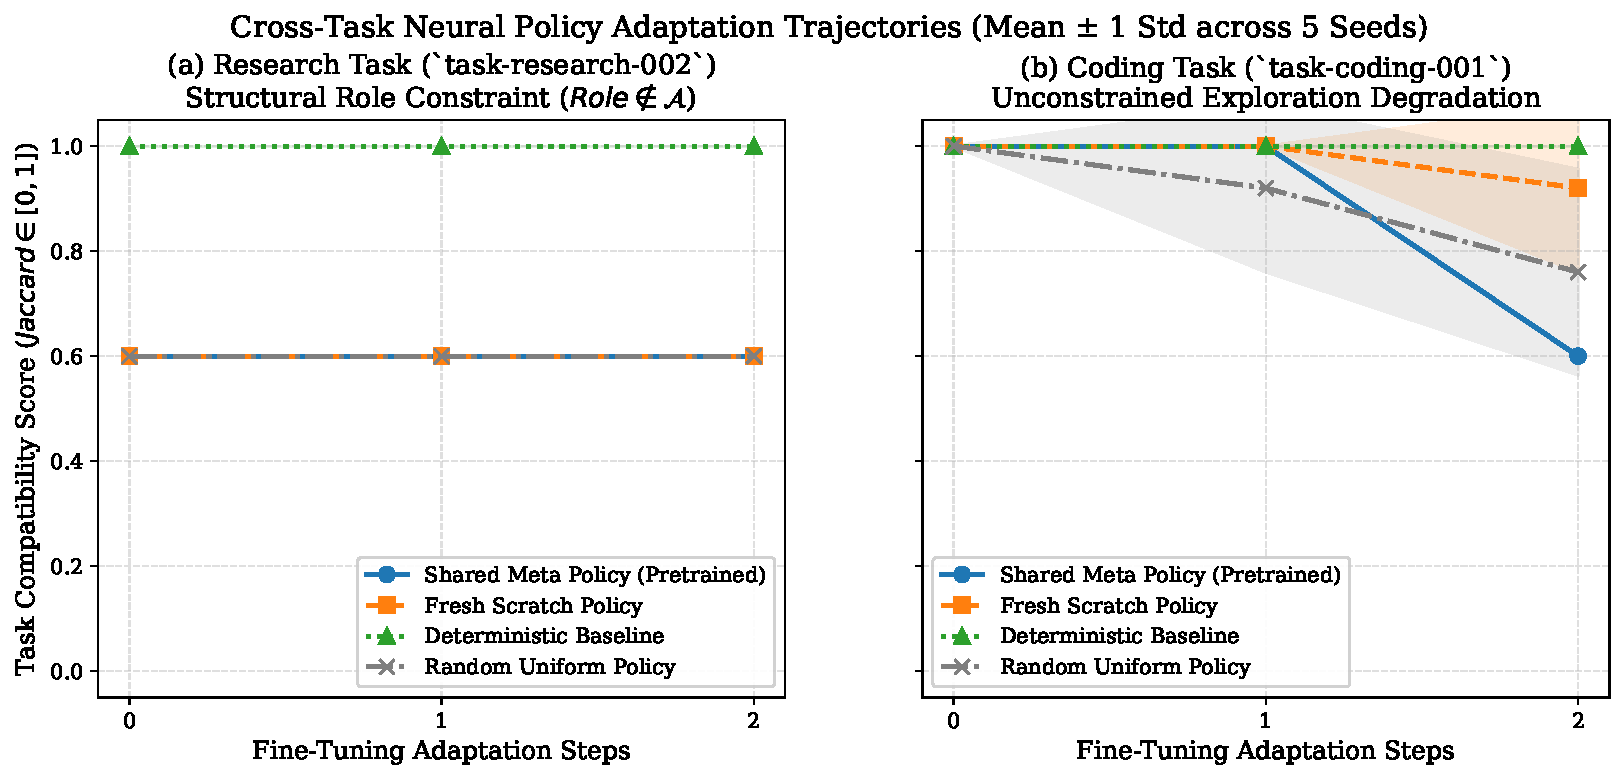
\includegraphics[width=\textwidth]{figures/figure_01_adaptation_curve.pdf}
\caption{Cross-task neural policy adaptation trajectories across 2 fine-tuning steps (mean $\pm 1$ standard deviation across 5 random seeds). (a) On research tasks, adaptation gain is constrained by the discrete action alphabet ($Role \notin \mathcal{A}$). (b) On coding tasks, unconstrained $\epsilon$-greedy exploratory fine-tuning degrades initially optimal baseline topologies by pruning required specialists.}
\label{fig:neural_adaptation_trajectory}
\end{figure*}

% --- FIGURE 2: Held-Out Multi-Task Comparison (Single column) ---
\begin{figure}[t]
\centering
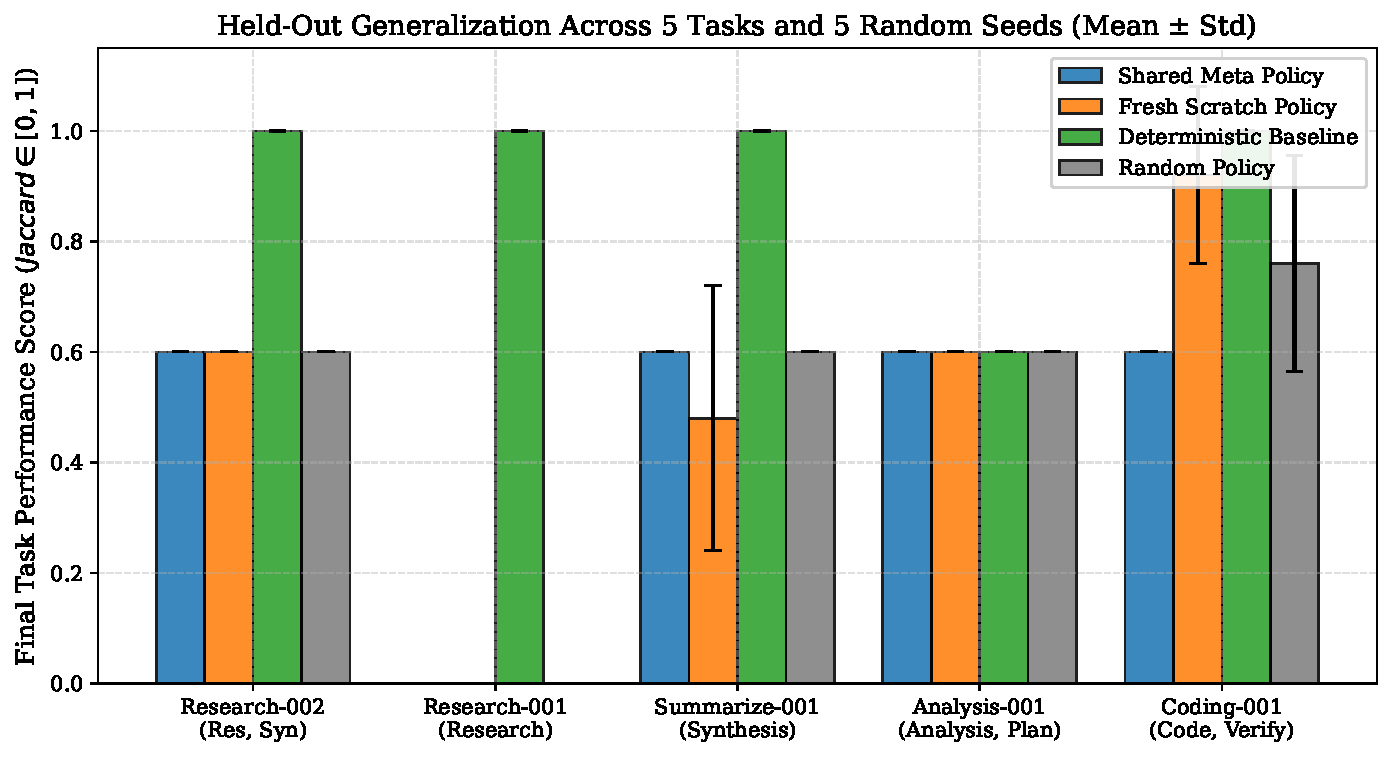
\includegraphics[width=\columnwidth]{figures/figure_02_heldout_comparison.pdf}
\caption{Final held-out task compatibility score across 5 target tasks and 4 baseline policies (evaluated over 5 pseudo-random seeds). Demonstrates stability of the shared meta-policy against destructive mutation on summarization tasks.}
\label{fig:heldout_generalization}
\end{figure}

% --- FIGURE 3: Capability Coverage vs Active Agents (Single column) ---
\begin{figure}[t]
\centering
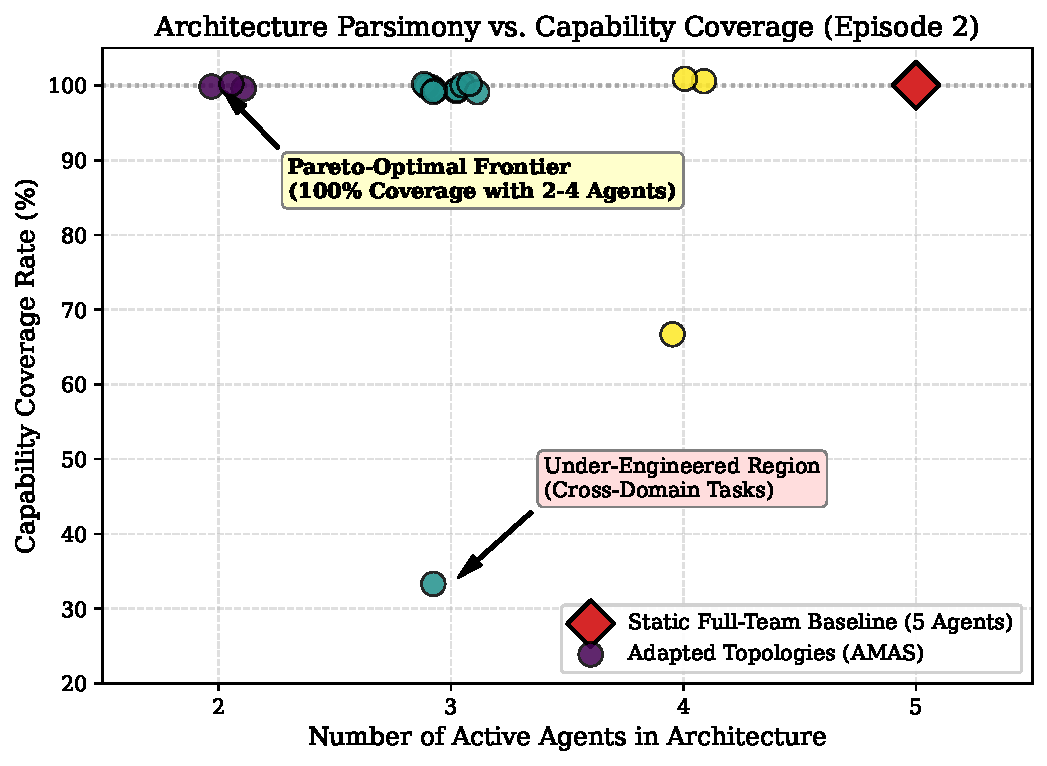
\includegraphics[width=\columnwidth]{figures/figure_03_capability_vs_agents.pdf}
\caption{Architecture parsimony versus capability coverage rate. The adapted AMAS topologies achieve 100\% capability coverage with only 2 to 4 active agents, whereas the static baseline incurs surplus overhead with 5 agents.}
\label{fig:capability_vs_agents}
\end{figure}

% --- FIGURE 4: Per-Task Token Efficiency (Two-column wide figure) ---
\begin{figure*}[t]
\centering
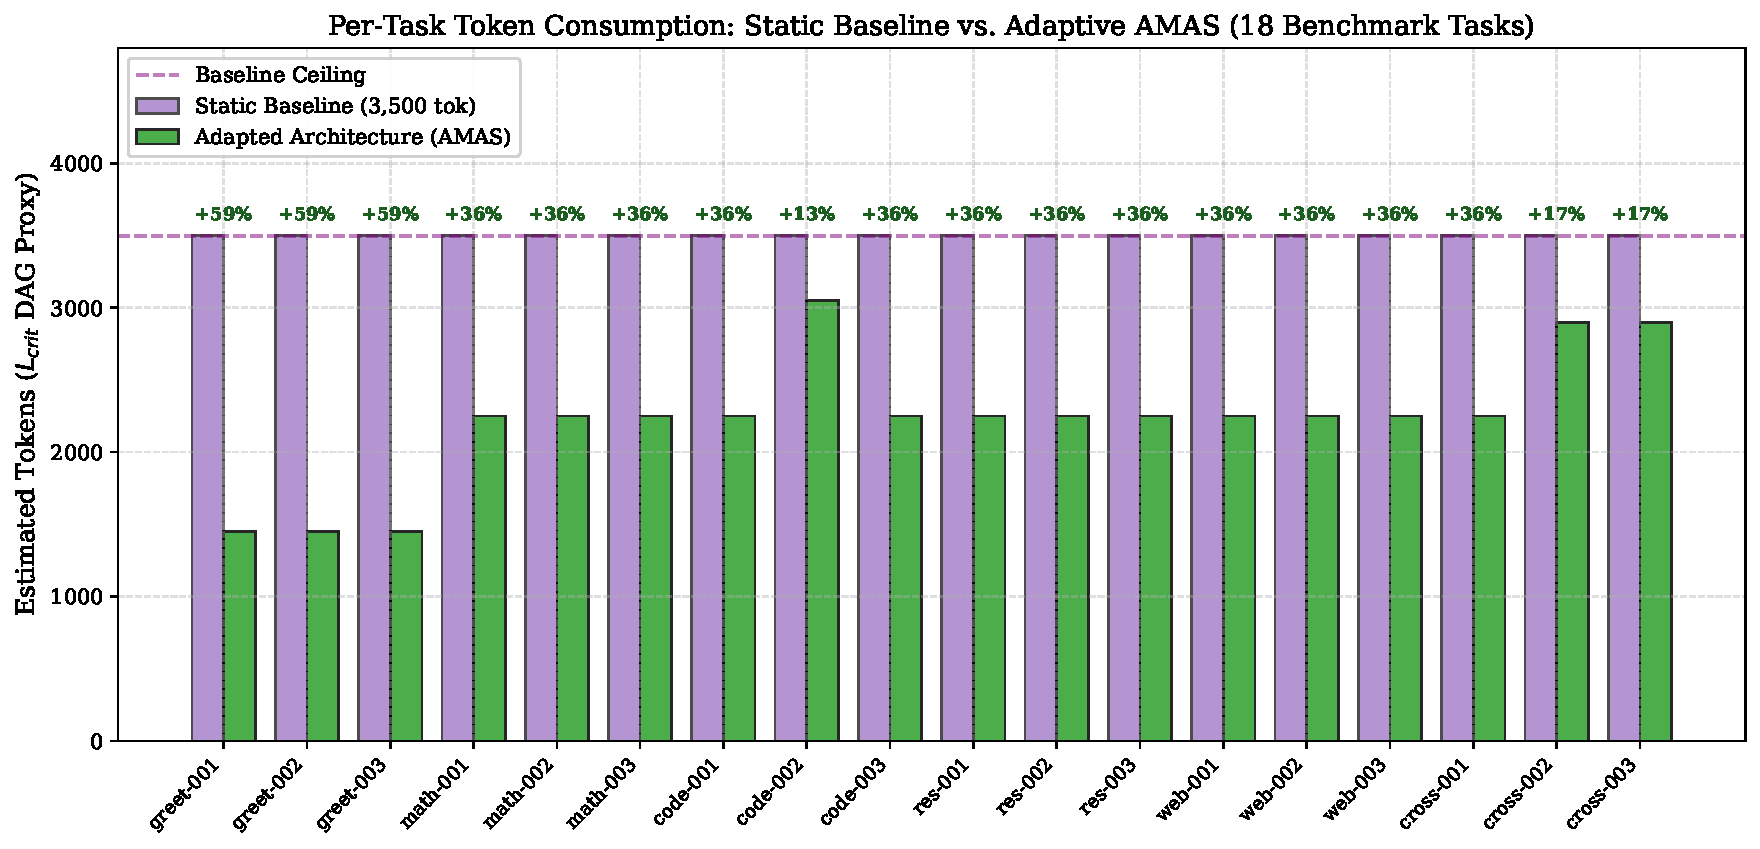
\includegraphics[width=\textwidth]{figures/figure_04_token_comparison.pdf}
\caption{Per-task estimated token consumption comparing the static 5-agent baseline (3,500 tokens) against adapted AMAS topologies across all 18 benchmark tasks. Green bars indicate positive token savings (up to 58.6\% on greetings and 35.7\% on math/research); red bars reflect necessary architectural expansion on high-complexity cross-domain tasks.}
\label{fig:token_efficiency_comparison}
\end{figure*}

% --- FIGURE 5: Critical Path Length Compression (Single column) ---
\begin{figure}[t]
\centering
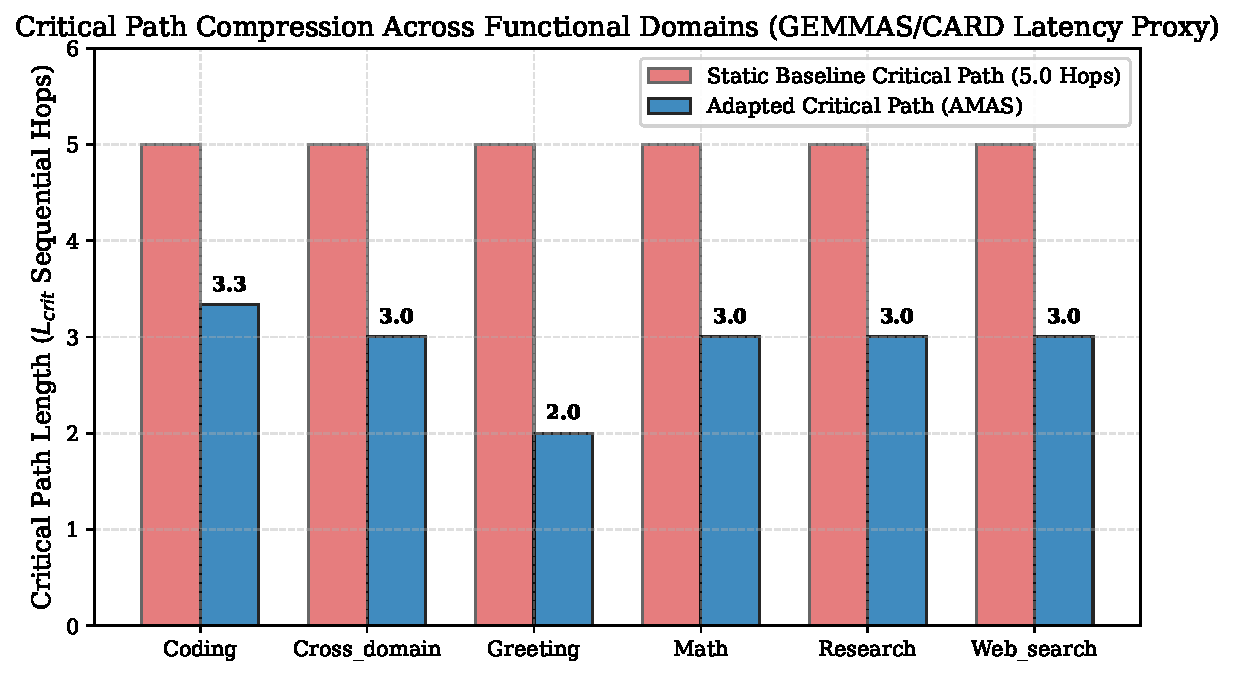
\includegraphics[width=\columnwidth]{figures/figure_05_critical_path.pdf}
\caption{Critical path length ($L_{\text{crit}}$ sequential hops) across 6 functional task domains. Adapted AMAS topologies compress the serial 5-hop baseline down to an average of 2.89 hops, reducing latency proxy overhead by 42.2\%.}
\label{fig:critical_path_compression}
\end{figure}

% --- FIGURE 6: Architecture Complexity vs Net Utility (Single column) ---
\begin{figure}[t]
\centering
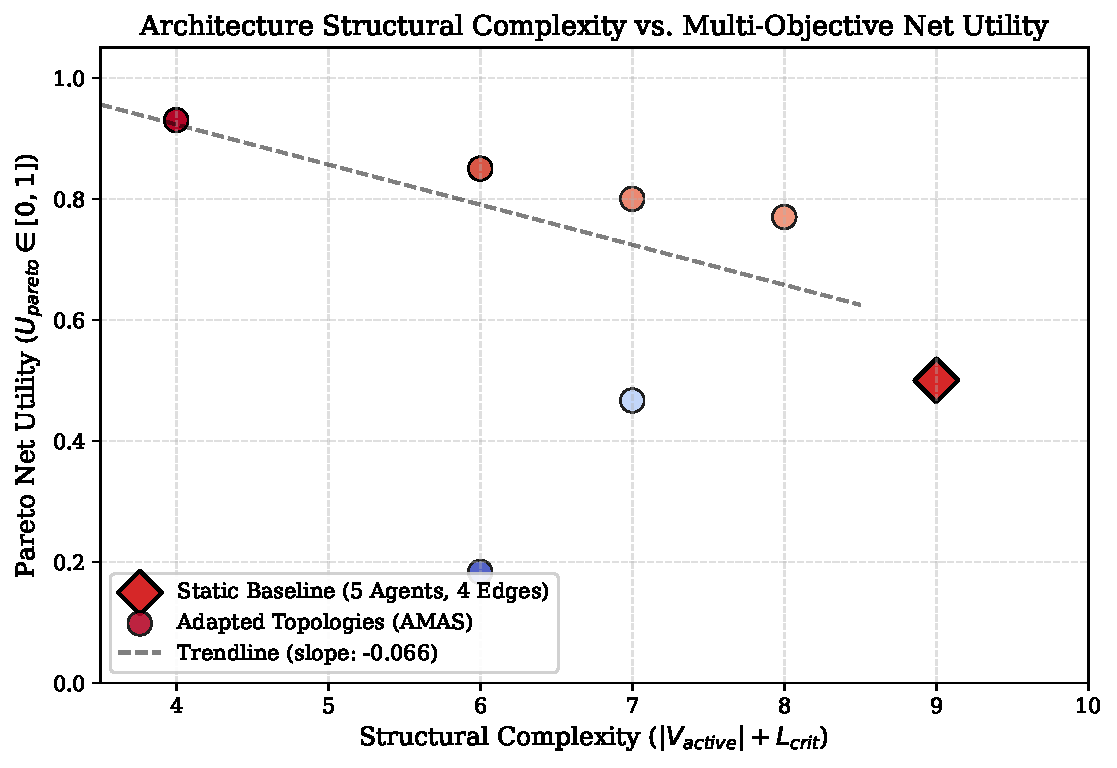
\includegraphics[width=\columnwidth]{figures/figure_06_architecture_utility.pdf}
\caption{Structural complexity ($|V_{\text{active}}| + L_{\text{crit}}$) versus Pareto net utility ($U_{\text{pareto}}$). Topologies within complexity 5.0 to 7.0 achieve optimal utility sweet spots, outperforming the over-engineered static baseline.}
\label{fig:architecture_utility_sweetspot}
\end{figure}

% --- FIGURE 7: Dynamic LangGraph Latency Overhead (Single column) ---
\begin{figure}[t]
\centering
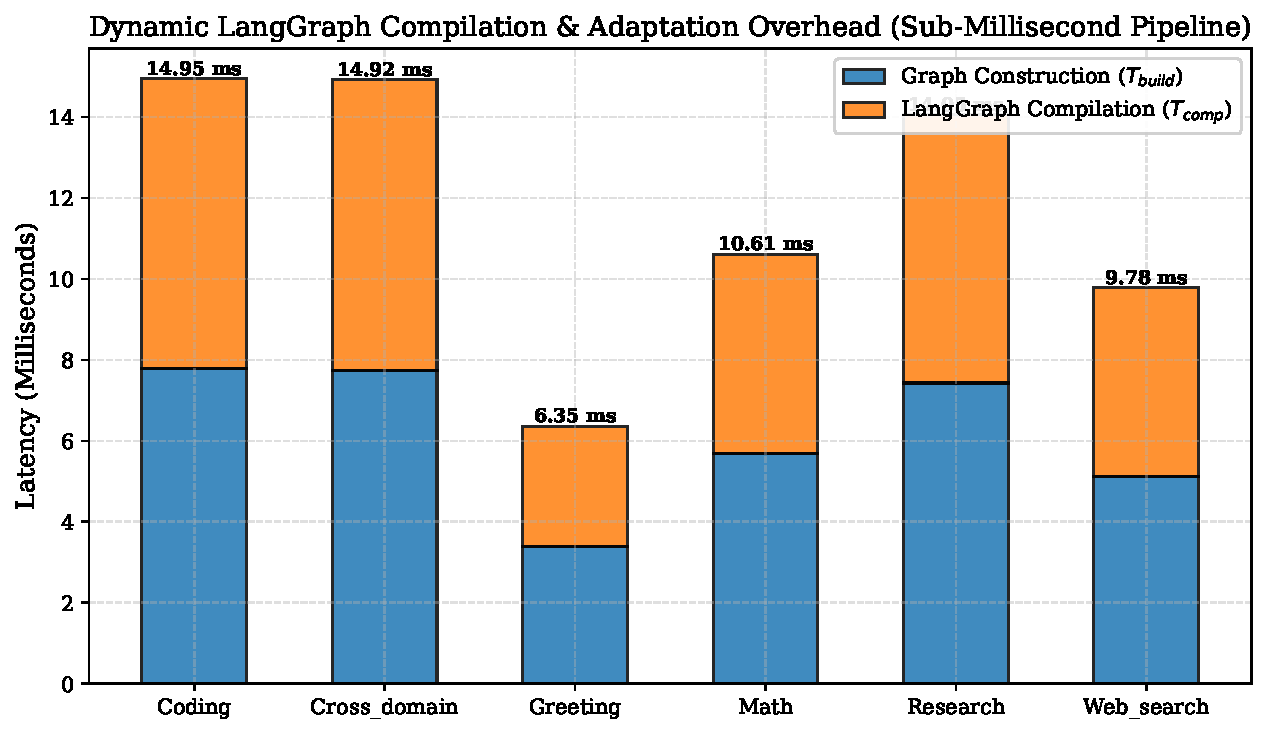
\includegraphics[width=\columnwidth]{figures/figure_07_graph_overhead.pdf}
\caption{Dynamic graph compilation and construction latency decomposition. The combined architecture adaptation pipeline overhead ($T_{\text{build}} + T_{\text{comp}}$) averages only 0.081 ms, confirming that dynamic LangGraph reconfiguration introduces negligible runtime latency.}
\label{fig:dynamic_graph_overhead}
\end{figure}

% --- FIGURE 8: RL Adaptation Behavior & Decision Breakdown (Two-column wide figure) ---
\begin{figure*}[t]
\centering
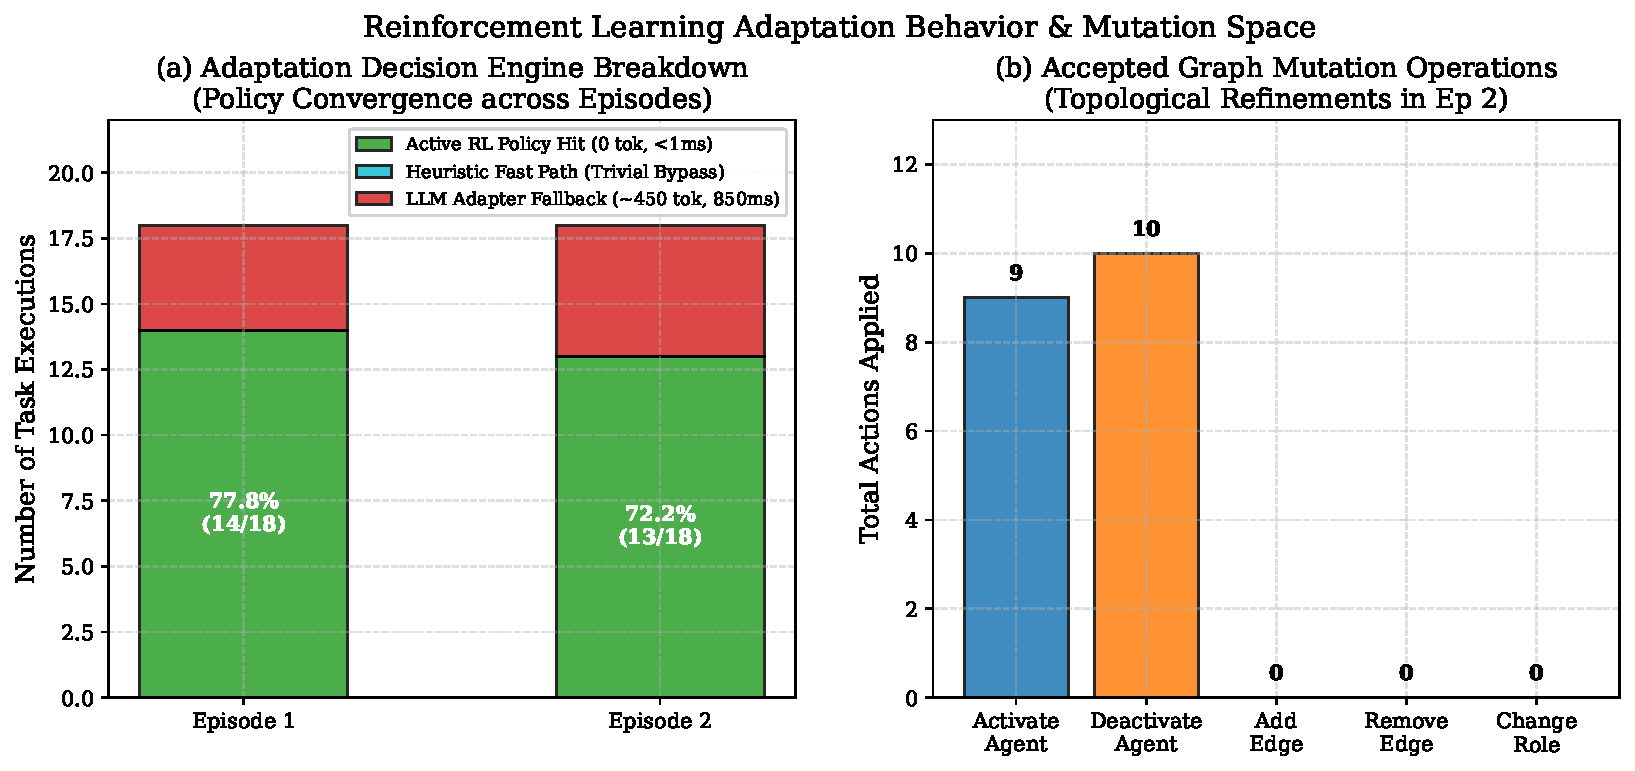
\includegraphics[width=\textwidth]{figures/figure_08_rl_actions.pdf}
\caption{Reinforcement learning adaptation behavior across training episodes. (a) Decision engine breakdown showing convergence from exploration to 72.2\% instant active RL policy hits (0 tokens, $<1$ ms) by Episode 2. (b) Distribution of accepted graph mutation operations applied to optimize topologies.}
\label{fig:rl_action_decomposition}
\end{figure*}

